
%(BEGIN_QUESTION)
% Copyright 2012, Tony R. Kuphaldt, released under den Creative Commons Attribution License (v 1.0)
% This means you may do almost anything med denne work of mine, so long as you give me proper credit

En nyinstallert {\sl Wireless}HART-temperaturtransmitter (TT-34), plassert langt fra Gateway eller andre {\sl Wireless}HART-enheter, har kommunikasjonsproblemer mot Gateway på grunn av avstand og signalstyrke. Signalveien mellom TT-34 og Gateway er fri for hindringer. Én løsning ville vært å installere flere {\sl Wireless}HART-enheter som repeatere mellom TT-34 og Gateway, men det er ikke tid til å bestille og installere nytt utstyr:

$$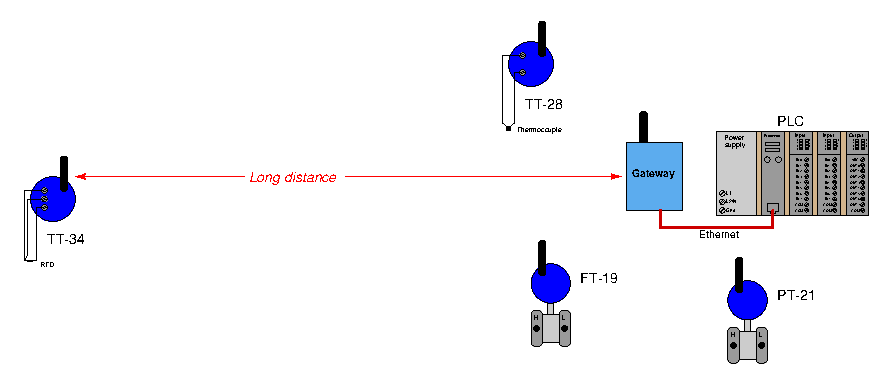
\includegraphics[width=15.5cm]{i01223x01.eps}$$

Beskriv én løsning som kan forbedre kommunikasjonen til TT-34, og som kan gjennomføres uten å bestille nye radiokomponenter (f.eks. nye antenner, flere {\sl Wireless}HART-enheter osv.).

\underbar{file i01223}
%(END_QUESTION)





%(BEGIN_ANSWER)

Full uttelling gis for svar som disse:

\begin{itemize}
\item{} Plassere en metallplate som ``reflektor'' til venstre for TT-34-antennen for å gjøre antennen mer retningsbestemt og øke antenneforsterkningen.
\item{} Flytte TT-34 til høyere plassering (dette krever forlengelse av RTD-ledningene slik at RTD-sensoren kan stå i samme prosesspunkt).
\item{} Flytte Gateway nærmere TT-34 (dette krever forlengelse av Ethernet-kabel, som normalt er praktisk gjennomførbart).
\end{itemize}

\vskip 10pt

Halv uttelling gis for mindre praktiske løsninger:

\begin{itemize}
\item{} Flytte TT-34 nærmere Gateway (dette krever ofte {\it lang} forlengelse av RTD-kabling, og gevinsten av redusert avstand er ofte mindre enn gevinsten av økt høyde).
\end{itemize}

%(END_ANSWER)





%(BEGIN_NOTES)

{\bf Denne oppgaven er kun ment for prøver/eksamen, ikke arbeidsark!}

%(END_NOTES)

